\begin{problem}[Line Intersection in 3D]
Find the intersection point of lines $\mathbf{r} = \begin{pmatrix} 3 \\ -1 \\ 7 \end{pmatrix} + \lambda \begin{pmatrix} 1 \\ 2 \\ 1 \end{pmatrix}$ and $\mathbf{r} = \begin{pmatrix} 1 \\ -6 \\ 2 \end{pmatrix} + \mu \begin{pmatrix} -2 \\ 1 \\ 3 \end{pmatrix}$.
\end{problem}

\begin{hint}
Set up three equations by equating components, then solve for parameters.
\end{hint}

\begin{solution}[Sketch]
Equating components: $3 + \lambda = 1 - 2\mu$, $-1 + 2\lambda = -6 + \mu$, $7 + \lambda = 2 + 3\mu$. From equations 1 and 3: $\lambda = -2\mu$ and $\lambda = -5 + 3\mu$. Solving: $\mu = 1$, $\lambda = -2$. Verify in equation 2. Intersection point: $(1, -5, 5)$.
\end{solution}

\vspace{1em}
\begin{problem}[Triangular Pyramid — Find Vertex Coordinates]
The diagram below shows a triangular pyramid with vertices 
$O(0,0,0)$, $P(4,3,0)$, $Q(3,4,0)$ and $R(x,y,z)$, 
where $x,y,z$ are positive real numbers. 
Given that $\angle RPO=\angle RQO=\frac{\pi}{3}$ and $|\vec{PR}|=|\vec{QR}|=5$, 
find the coordinates of $R$.


\tdplotsetmaincoords{70}{110}
\begin{center}
\begin{tikzpicture}[tdplot_main_coords, scale=0.8]
    % Axes
    \draw[thick,->] (0,0,0) -- (7,0,0) node[anchor=north east]{$x$};
    \draw[thick,->] (0,0,0) -- (0,7,0) node[anchor=north west]{$y$};
    \draw[thick,->] (0,0,0) -- (0,0,7) node[anchor=south]{$z$};

    % Points
    \coordinate (O) at (0,0,0);
    \coordinate (P) at (4,3,0);
    \coordinate (Q) at (3,4,0);
    \coordinate (R) at (1.78, 1.78, 4.35); % Approximate for visualization

    % Lines - Solid for visible
    \draw[thick, blue] (O) -- (P) node[midway, below left] {5};
    \draw[thick, blue] (O) -- (Q) node[midway, below right] {5};
    \draw[thick, blue] (P) -- (Q);
    \draw[thick, blue] (O) -- (R);
    \draw[thick, blue] (P) -- (R) node[midway, left] {5};
    \draw[thick, blue] (Q) -- (R) node[midway, right] {5};

    % Labels
    \node[anchor=south east] at (O) {$O(0,0,0)$};
    \node[anchor=north] at (P) {$P(4,3,0)$};
    \node[anchor=west] at (Q) {$Q(3,4,0)$};
    \node[anchor=south west] at (R) {$R(x,y,z)$};

    % Angles (Arcs)
    % Angle RPO
    \draw[thin, blue] (4,3,0) ++(140:0.8) arc (140:100:0.8);
    \node[blue, scale=0.8] at (3.5, 3.2, 0.5) {$\frac{\pi}{3}$};
    
    % Angle RQO
    \draw[thin, blue] (3,4,0) ++(120:0.8) arc (120:80:0.8);
    \node[blue, scale=0.8] at (2.8, 3.5, 0.5) {$\frac{\pi}{3}$};

    % Dashed lines for projection (optional, adds depth)
    \draw[dashed, gray] (R) -- (1.78, 1.78, 0);
\end{tikzpicture}
\end{center}


\end{problem}

\begin{hint}
\begin{itemize}
    \item Calculate $|OP|$ and $|OQ|$ to recognise any special triangle.
    \item Use the fact that equal sides with included $60^\circ$ imply equilateral properties.
    \item Set up three sphere-distance equations for $R(x,y,z)$ from $O,P,Q$ and subtract to get linear relations for $x,y$.
\end{itemize}
\end{hint}

\begin{solution}[Sketch]
Compute $|OP|=\sqrt{4^2+3^2}=5$ and $|OQ|=5$. Since $|PR|=5$ and $\angle RPO=60^\circ$, triangle $RPO$ is equilateral so $|OR|=5$. Thus
\begin{align*}
x^2+y^2+z^2 &= 25, \\
(x-4)^2+(y-3)^2+z^2 &= 25, \\
(x-3)^2+(y-4)^2+z^2 &= 25.
\end{align*}
Subtracting the first from the second and third gives the linear system
\begin{align*}
8x+6y &= 25, \\
6x+8y &= 25,
\end{align*}
so by symmetry $x=y=\tfrac{25}{14}$. Substituting into $x^2+y^2+z^2=25$ yields $z=\dfrac{5\sqrt{47}}{7}$.
\end{solution}

\vspace{0.5em}
\noindent\textbf{Takeaways}
\begin{itemize}
    \item Intersection of spheres often reduces 3D location problems to solving linear systems by subtraction.
    \item Symmetry in the base points can force $x=y$ and simplify algebra.
\end{itemize}

\begin{problem}[Perpendicular Intersecting Lines]
Consider the line $L_1: \mathbf{r} = \begin{pmatrix} 3 \\ -1 \\ 7 \end{pmatrix} + \mu \begin{pmatrix} 1 \\ 2 \\ 1 \end{pmatrix}$ and the line $L_2: \mathbf{r} = \begin{pmatrix} 1 \\ 0 \\ p \end{pmatrix} + \lambda \begin{pmatrix} 2 \\ q \\ -1 \end{pmatrix}$. \\
Given that these two lines intersect and are perpendicular to each other, find the values of $p$ and $q$. \\
(Note: Two conditions must be satisfied: the lines must intersect at some point, and their direction vectors must be perpendicular.)
\end{problem}

\begin{hint}
Use perpendicularity condition (dot product = 0) and intersection condition (solve system).
\end{hint}

\begin{solution}[Sketch]
\textbf{Step 1: Find $q$ from perpendicularity.} Direction vectors: $\mathbf{d}_1 = (1, 2, 1)$ and $\mathbf{d}_2 = (2, q, -1)$. Since $\mathbf{d}_1 \cdot \mathbf{d}_2 = 0$: $(1)(2) + (2)(q) + (1)(-1) = 0 \Rightarrow 2q = -1 \Rightarrow q = -\frac{1}{2}$.

\textbf{Step 2: Set up intersection condition.} The lines intersect when $\begin{pmatrix} 3 \\ -1 \\ 7 \end{pmatrix} + \mu \begin{pmatrix} 1 \\ 2 \\ 1 \end{pmatrix} = \begin{pmatrix} 1 \\ 0 \\ p \end{pmatrix} + \lambda \begin{pmatrix} 2 \\ -1/2 \\ -1 \end{pmatrix}$. This gives: $3 + \mu = 1 + 2\lambda$, $-1 + 2\mu = -\frac{1}{2}\lambda$, and $7 + \mu = p - \lambda$.

\textbf{Step 3: Solve for $\mu$ and $\lambda$.} From first equation: $\mu = 2\lambda - 2$. Substituting into second: $-1 + 2(2\lambda - 2) = -\frac{1}{2}\lambda \Rightarrow \frac{9}{2}\lambda = 5 \Rightarrow \lambda = \frac{10}{9}$. Thus $\mu = \frac{2}{9}$.

\textbf{Step 4: Find $p$.} From third equation: $p = 7 + \frac{2}{9} + \frac{10}{9} = 7 + \frac{4}{3} = \frac{25}{3}$.

\textbf{Answer:} $p = \dfrac{25}{3}$ and $q = -\dfrac{1}{2}$.
\end{solution}

\vspace{1em}

\begin{problem}[Tetrahedron Collinearity]
\begin{enumerate}[label=(\roman*)]
    \item The two non-parallel vectors $\vec{u}$ and $\vec{v}$ satisfy $\lambda \vec{u} + \mu \vec{v} = \vec{0}$ for some real numbers $\lambda$ and $\mu$.
    
    Show that $\lambda = \mu = 0$.

    \item The two non-parallel vectors $\vec{u}$ and $\vec{v}$ satisfy $\lambda_1 \vec{u} + \mu_1 \vec{v} = \lambda_2 \vec{u} + \mu_2 \vec{v}$ for some real numbers $\lambda_1, \lambda_2, \mu_1$ and $\mu_2$.
    
    Using part (i), or otherwise, show that $\lambda_1 = \lambda_2$ and $\mu_1 = \mu_2$.
\end{enumerate}


\vspace{0.3cm}

\noindent The diagram below shows a tetrahedron with vertices $A, B, C$ and $S$.

\noindent The point $K$ is defined by $\vec{SK} = \frac{1}{4}\vec{SB} + \frac{1}{3}\vec{SC}$, as shown in the diagram.

\noindent The point $L$ is the point of intersection of the straight lines $SK$ and $BC$.

\vspace{0.3cm}

\begin{center}
\begin{tikzpicture}[scale=1.2, cap=round, join=round]
    % Define coordinates
    \coordinate (S) at (2, 3.5);
    \coordinate (A) at (0, 0);
    \coordinate (B) at (4, -0.3);
    \coordinate (C) at (5, 1.2);

    % Calculate L based on BL = 4/7 BC
    \coordinate (L) at ($(B)!4/7!(C)$);

    % Calculate K based on SK = 1/4 SB + 1/3 SC
    \coordinate (K) at ($(S) + 0.25*($(B)-(S)$) + 0.3333*($(C)-(S)$)$);

    % Dashed lines for hidden edges
    \draw[dashed] (A) -- (C);
    \draw[dashed] (A) -- (L);

    % Main Tetrahedron Edges
    \draw (S) -- (A);
    \draw (S) -- (B);
    \draw (S) -- (C);
    \draw (A) -- (B);
    \draw (B) -- (C);
    
    % Lines SK and KL
    \draw (S) -- (K);
    \draw (K) -- (L);

    % Points
    \fill (S) circle (1.2pt) node[above] {$S$};
    \fill (A) circle (1.2pt) node[left] {$A$};
    \fill (B) circle (1.2pt) node[below] {$B$};
    \fill (C) circle (1.2pt) node[right] {$C$};
    \fill (K) circle (1.2pt) node[right=2pt] {$K$};
    \fill (L) circle (1.2pt) node[below right=1pt] {$L$};
\end{tikzpicture}
\end{center}

\vspace{0.3cm}

\begin{enumerate}[resume*, label=(\roman*)]
    \item Using part (ii), or otherwise, determine the position of $L$ by showing that $\vec{BL} = \frac{4}{7}\vec{BC}$.
    
    \item The point $P$ is defined by $\vec{AP} = -6\vec{AB} - 8\vec{AC}$.
    
    Does $P$ lie on the line $AL$? Justify your answer.
\end{enumerate}
\end{problem}

\begin{hint}
(i) Use proof by contradiction: if $\lambda \neq 0$, then $\vec{u} = -\frac{\mu}{\lambda}\vec{v}$, contradicting non-parallel assumption. 
(ii) Rearrange to get $(\lambda_1 - \lambda_2)\vec{u} + (\mu_1 - \mu_2)\vec{v} = \vec{0}$ and apply part (i).
(iii) Express $\vec{SL}$ in two ways: as $m\vec{SK}$ and as $(1-k)\vec{SB} + k\vec{SC}$, then equate coefficients.
(iv) Express $\vec{AL}$ in terms of $\vec{AB}$ and $\vec{AC}$, then check if $\vec{AP} = c\vec{AL}$ for some scalar $c$.
\end{hint}

\begin{solution}[Sketch]
(i) Assume $\lambda \neq 0$. Then $\vec{u} = -\frac{\mu}{\lambda}\vec{v}$, implying $\vec{u} \parallel \vec{v}$, contradiction. Thus $\lambda = 0$, which gives $\mu = 0$.

(ii) Rearranging: $(\lambda_1 - \lambda_2)\vec{u} + (\mu_1 - \mu_2)\vec{v} = \vec{0}$. By part (i), both coefficients equal zero.

(iii) Since $S, K, L$ are collinear: $\vec{SL} = m\vec{SK} = \frac{m}{4}\vec{SB} + \frac{m}{3}\vec{SC}$. Since $L$ is on $BC$: $\vec{SL} = (1-k)\vec{SB} + k\vec{SC}$ where $\vec{BL} = k\vec{BC}$. Equating coefficients: $\frac{m}{4} = 1-k$ and $\frac{m}{3} = k$. Solving: $m = \frac{12}{7}$ and $k = \frac{4}{7}$.

(iv) $\vec{AL} = \vec{AB} + \frac{4}{7}\vec{BC} = \vec{AB} + \frac{4}{7}(\vec{AC} - \vec{AB}) = \frac{3}{7}\vec{AB} + \frac{4}{7}\vec{AC}$. Check: $\vec{AP} = -6\vec{AB} - 8\vec{AC} = -14(\frac{3}{7}\vec{AB} + \frac{4}{7}\vec{AC}) = -14\vec{AL}$. Yes, $P$ lies on line $AL$ (extended backwards through $A$).
\end{solution}

\vspace{1em}

\begin{problem}[Varignon's Theorem - Midpoint Parallelogram]
Let $ABCD$ be any quadrilateral in three-dimensional space (not necessarily planar). Let $P$, $Q$, $R$, and $S$ be the midpoints of sides $AB$, $BC$, $CD$, and $DA$ respectively.

\begin{center}
\begin{tikzpicture}[scale=0.85]
    % CONVEX QUADRILATERAL
    \begin{scope}[xshift=0cm]
        % Define coordinates for a convex quadrilateral
        \coordinate (A) at (0, 0);
        \coordinate (B) at (3, -0.3);
        \coordinate (C) at (3.5, 2.3);
        \coordinate (D) at (0.3, 2.5);
        
        % Calculate midpoints
        \coordinate (P) at ($(A)!0.5!(B)$);
        \coordinate (Q) at ($(B)!0.5!(C)$);
        \coordinate (R) at ($(C)!0.5!(D)$);
        \coordinate (S) at ($(D)!0.5!(A)$);
        
        % Draw the original quadrilateral ABCD
        \draw[thick, black!70] (A) -- (B) -- (C) -- (D) -- cycle;
        
        % Fill the midpoint parallelogram
        \fill[red!15] (P) -- (Q) -- (R) -- (S) -- cycle;
        
        % Draw the midpoint parallelogram PQRS
        \draw[thick, red!70] (P) -- (Q) -- (R) -- (S) -- cycle;
        
        % Label the vertices of ABCD
        \fill[blue] (A) circle (1.5pt);
        \fill[blue] (B) circle (1.5pt);
        \fill[blue] (C) circle (1.5pt);
        \fill[blue] (D) circle (1.5pt);
        \node[below left, blue] at (A) {$A$};
        \node[below right, blue] at (B) {$B$};
        \node[above right, blue] at (C) {$C$};
        \node[above left, blue] at (D) {$D$};
        
        % Label the midpoints P, Q, R, S
        \fill[red] (P) circle (1.5pt);
        \fill[red] (Q) circle (1.5pt);
        \fill[red] (R) circle (1.5pt);
        \fill[red] (S) circle (1.5pt);
        \node[below, red, font=\small] at (P) {$P$};
        \node[right, red, font=\small] at (Q) {$Q$};
        \node[above, red, font=\small] at (R) {$R$};
        \node[left, red, font=\small] at (S) {$S$};
        
        % Title
        \node[font=\small\bfseries] at (1.75, 3.2) {convex quadrilateral};
    \end{scope}
    
    % CONCAVE QUADRILATERAL
    \begin{scope}[xshift=5.5cm]
        % Define coordinates for a concave quadrilateral
        \coordinate (A) at (0, 0);
        \coordinate (B) at (1.2, 1.5);
        \coordinate (C) at (4, 0.3);
        \coordinate (D) at (0.3, 2.5);
        
        % Calculate midpoints
        \coordinate (P) at ($(A)!0.5!(B)$);
        \coordinate (Q) at ($(B)!0.5!(C)$);
        \coordinate (R) at ($(C)!0.5!(D)$);
        \coordinate (S) at ($(D)!0.5!(A)$);
        
        % Draw the original quadrilateral ABCD
        \draw[thick, black!70] (A) -- (B) -- (C) -- (D) -- cycle;
        
        % Fill the midpoint parallelogram
        \fill[red!15] (P) -- (Q) -- (R) -- (S) -- cycle;
        
        % Draw the midpoint parallelogram PQRS
        \draw[thick, red!70] (P) -- (Q) -- (R) -- (S) -- cycle;
        
        % Label the vertices of ABCD
        \fill[blue] (A) circle (1.5pt);
        \fill[blue] (B) circle (1.5pt);
        \fill[blue] (C) circle (1.5pt);
        \fill[blue] (D) circle (1.5pt);
        \node[below, blue] at (A) {$A$};
        \node[above left, blue] at (B) {$B$};
        \node[below right, blue] at (C) {$C$};
        \node[above left, blue] at (D) {$D$};
        
        % Label the midpoints P, Q, R, S
        \fill[red] (P) circle (1.5pt);
        \fill[red] (Q) circle (1.5pt);
        \fill[red] (R) circle (1.5pt);
        \fill[red] (S) circle (1.5pt);
        \node[left, red, font=\small] at (P) {$P$};
        \node[above right, red, font=\small] at (Q) {$Q$};
        \node[right, red, font=\small] at (R) {$R$};
        \node[left, red, font=\small] at (S) {$S$};
        
        % Title
        \node[font=\small\bfseries] at (2, 3.2) {concave quadrilateral};
    \end{scope}
    
    % CROSSED QUADRILATERAL
    \begin{scope}[xshift=11cm]
        % Define coordinates for a crossed quadrilateral
        \coordinate (A) at (0, 0);
        \coordinate (B) at (0.3, 2.5);
        \coordinate (C) at (3.5, -0.3);
        \coordinate (D) at (0.5, 1.2);
        
        % Calculate midpoints
        \coordinate (P) at ($(A)!0.5!(B)$);
        \coordinate (Q) at ($(B)!0.5!(C)$);
        \coordinate (R) at ($(C)!0.5!(D)$);
        \coordinate (S) at ($(D)!0.5!(A)$);
        
        % Draw the original quadrilateral ABCD
        \draw[thick, black!70] (A) -- (B) -- (C) -- (D) -- cycle;
        
        % Fill the midpoint parallelogram
        \fill[red!15] (P) -- (Q) -- (R) -- (S) -- cycle;
        
        % Draw the midpoint parallelogram PQRS
        \draw[thick, red!70] (P) -- (Q) -- (R) -- (S) -- cycle;
        
        % Label the vertices of ABCD
        \fill[blue] (A) circle (1.5pt);
        \fill[blue] (B) circle (1.5pt);
        \fill[blue] (C) circle (1.5pt);
        \fill[blue] (D) circle (1.5pt);
        \node[below, blue] at (A) {$A$};
        \node[above left, blue] at (B) {$B$};
        \node[below right, blue] at (C) {$C$};
        \node[left, blue] at (D) {$D$};
        
        % Label the midpoints P, Q, R, S
        \fill[red] (P) circle (1.5pt);
        \fill[red] (Q) circle (1.5pt);
        \fill[red] (R) circle (1.5pt);
        \fill[red] (S) circle (1.5pt);
        \node[left, red, font=\small] at (P) {$P$};
        \node[above right, red, font=\small] at (Q) {$Q$};
        \node[below right, red, font=\small] at (R) {$R$};
        \node[left, red, font=\small] at (S) {$S$};
        
        % Title
        \node[font=\small\bfseries] at (1.75, 3.2) {crossed quadrilateral};
    \end{scope}
\end{tikzpicture}
\end{center}

\vspace{0.5em}

\textit{3D Non-Planar Quadrilateral:}

\begin{center}
\begin{tikzpicture}[scale=1.2, x={(0.8cm, 0.4cm)}, y={(0cm, 1cm)}, z={(-0.6cm, 0.3cm)}]
    % Annotation on the left
    \node[font=\small, align=right, anchor=east] at (-1, 1.5, 1.5) {Non-planar quadrilateral\\in $\mathbb{R}^3$\\{\footnotesize (vertices not in}\\{\footnotesize the same plane)}};
    
    % Define 3D coordinates for a non-planar quadrilateral
    % A at top, B, C, D form the base
    \coordinate (A) at (1.5, 3, 1);
    \coordinate (B) at (0, 0, 0);
    \coordinate (C) at (3, 0, 0);
    \coordinate (D) at (1.5, 0, 2.5);
    
    % Calculate midpoints
    \coordinate (P) at ($(A)!0.5!(B)$);
    \coordinate (Q) at ($(B)!0.5!(C)$);
    \coordinate (R) at ($(C)!0.5!(D)$);
    \coordinate (S) at ($(D)!0.5!(A)$);
    
    % Draw back edges (dotted - invisible from viewer)
    \draw[thick, black!50, dotted] (B) -- (D);
    \draw[thick, black!50, dotted] (A) -- (D);
    
    % Draw the midpoint parallelogram (with fill)
    \fill[red!15, opacity=0.7] (P) -- (Q) -- (R) -- (S) -- cycle;
    \draw[thick, red!70] (P) -- (Q) -- (R) -- (S) -- cycle;
    
    % Draw front edges (solid)
    \draw[thick, black!70] (A) -- (B);
    \draw[thick, black!70] (B) -- (C);
    \draw[thick, black!70] (C) -- (D);
    \draw[thick, black!70] (A) -- (C);
    
    % Draw axes for reference (light gray, dashed)
    \draw[gray!40, dashed, ->] (0, 0, 0) -- (3.5, 0, 0) node[right, font=\tiny] {$x$};
    \draw[gray!40, dashed, ->] (0, 0, 0) -- (0, 3.5, 0) node[above, font=\tiny] {$y$};
    \draw[gray!40, dashed, ->] (0, 0, 0) -- (0, 0, 3) node[below left, font=\tiny] {$z$};
    
    % Label the vertices of ABCD
    \fill[blue] (A) circle (1.5pt);
    \fill[blue] (B) circle (1.5pt);
    \fill[blue] (C) circle (1.5pt);
    \fill[blue] (D) circle (1.5pt);
    \node[above, blue] at (A) {$A$};
    \node[below left, blue] at (B) {$B$};
    \node[below right, blue] at (C) {$C$};
    \node[below, blue] at (D) {$D$};
    
    % Label the midpoints P, Q, R, S
    \fill[red] (P) circle (1.5pt);
    \fill[red] (Q) circle (1.5pt);
    \fill[red] (R) circle (1.5pt);
    \fill[red] (S) circle (1.5pt);
    \node[left, red, font=\small] at (P) {$P$};
    \node[below, red, font=\small] at (Q) {$Q$};
    \node[right, red, font=\small] at (R) {$R$};
    \node[above right, red, font=\small] at (S) {$S$};
\end{tikzpicture}
\end{center}

\begin{enumerate}[label=(\roman*)]
    \item Express the position vectors of $P$, $Q$, $R$, and $S$ in terms of the position vectors $\mathbf{a}$, $\mathbf{b}$, $\mathbf{c}$, and $\mathbf{d}$ of points $A$, $B$, $C$, and $D$ respectively.
    
    \item Show that $\overrightarrow{PQ} = \overrightarrow{SR}$.
    
    \item Hence, prove that $PQRS$ is a parallelogram.
    
    \item If $ABCD$ is a parallelogram, what special type of quadrilateral is $PQRS$? Justify your answer.
\end{enumerate}

\textit{Note: This result is known as Varignon's Theorem (1731). It states that the midpoints of any quadrilateral always form a parallelogram, regardless of the shape of the original quadrilateral.}
\end{problem}

\begin{hint}
(i) Use the midpoint formula: the position vector of the midpoint of two points is the average of their position vectors.
(ii) Express both $\overrightarrow{PQ}$ and $\overrightarrow{SR}$ in terms of $\mathbf{a}$, $\mathbf{b}$, $\mathbf{c}$, and $\mathbf{d}$, then show they are equal.
(iii) Use the result from (ii) - if one pair of opposite sides is equal and parallel, then $PQRS$ is a parallelogram.
(iv) When $ABCD$ is a parallelogram, use $\overrightarrow{DC} = \overrightarrow{AB}$ and investigate the relationship between adjacent sides of $PQRS$.
\end{hint}

\begin{solution}[Sketch]
(i) Using the midpoint formula:
\begin{align*}
\mathbf{p} &= \frac{\mathbf{a} + \mathbf{b}}{2} \\
\mathbf{q} &= \frac{\mathbf{b} + \mathbf{c}}{2} \\
\mathbf{r} &= \frac{\mathbf{c} + \mathbf{d}}{2} \\
\mathbf{s} &= \frac{\mathbf{d} + \mathbf{a}}{2}
\end{align*}

(ii) Calculate $\overrightarrow{PQ}$:
\begin{align*}
\overrightarrow{PQ} &= \mathbf{q} - \mathbf{p} = \frac{\mathbf{b} + \mathbf{c}}{2} - \frac{\mathbf{a} + \mathbf{b}}{2} \\
&= \frac{\mathbf{b} + \mathbf{c} - \mathbf{a} - \mathbf{b}}{2} = \frac{\mathbf{c} - \mathbf{a}}{2}
\end{align*}

Calculate $\overrightarrow{SR}$:
\begin{align*}
\overrightarrow{SR} &= \mathbf{r} - \mathbf{s} = \frac{\mathbf{c} + \mathbf{d}}{2} - \frac{\mathbf{d} + \mathbf{a}}{2} \\
&= \frac{\mathbf{c} + \mathbf{d} - \mathbf{d} - \mathbf{a}}{2} = \frac{\mathbf{c} - \mathbf{a}}{2}
\end{align*}

Therefore $\overrightarrow{PQ} = \overrightarrow{SR}$.

(iii) Since $\overrightarrow{PQ} = \overrightarrow{SR}$, the sides $PQ$ and $SR$ are equal in length and parallel. By definition, a quadrilateral with one pair of opposite sides equal and parallel is a parallelogram. Therefore $PQRS$ is a parallelogram.

(iv) If $ABCD$ is a parallelogram, then $\overrightarrow{AB} = \overrightarrow{DC}$, which means $\mathbf{b} - \mathbf{a} = \mathbf{c} - \mathbf{d}$.

Calculate $\overrightarrow{PS}$:
$$\overrightarrow{PS} = \mathbf{s} - \mathbf{p} = \frac{\mathbf{d} + \mathbf{a}}{2} - \frac{\mathbf{a} + \mathbf{b}}{2} = \frac{\mathbf{d} - \mathbf{b}}{2}$$

Calculate $\overrightarrow{QR}$:
$$\overrightarrow{QR} = \mathbf{r} - \mathbf{q} = \frac{\mathbf{c} + \mathbf{d}}{2} - \frac{\mathbf{b} + \mathbf{c}}{2} = \frac{\mathbf{d} - \mathbf{b}}{2}$$

So $\overrightarrow{PS} = \overrightarrow{QR}$, meaning both pairs of opposite sides are equal and parallel.

Additionally, from (ii): $|\overrightarrow{PQ}| = \frac{1}{2}|\mathbf{c} - \mathbf{a}| = \frac{1}{2}|\overrightarrow{AC}|$ (half the diagonal $AC$).

Similarly: $|\overrightarrow{PS}| = \frac{1}{2}|\mathbf{d} - \mathbf{b}| = \frac{1}{2}|\overrightarrow{BD}|$ (half the diagonal $BD$).

If $ABCD$ is a parallelogram with equal diagonals, 
then $PQRS$ is a rhombus (all four sides equal). 
If the diagonals of $ABCD$ are perpendicular, then $PQRS$ is a rectangle.
\end{solution}

\vspace{1em}

\begin{problem}[Force Vector Analysis]
A particle is subject to two forces and undergoes a displacement in three-dimensional space.

\begin{enumerate}[label=(\roman*)]
    \item Force $\mathbf{F}_1$ has magnitude 12 newtons in the direction of vector $2\mathbf{i} - 2\mathbf{j} + \mathbf{k}$. 
    
    Show that $\mathbf{F}_1 = 8\mathbf{i} - 8\mathbf{j} + 4\mathbf{k}$ newtons.
    
    \item Force $\mathbf{F}_1$ from part (i) and a second force, $\mathbf{F}_2 = -6\mathbf{i} + 12\mathbf{j} + 4\mathbf{k}$ newtons, both act upon the particle. 
    
    Show that the resultant force acting on the particle is given by:
    $$\mathbf{F}_3 = 2\mathbf{i} + 4\mathbf{j} + 8\mathbf{k} \text{ newtons}$$
    
    \item The particle moves through a displacement $\mathbf{d} = \mathbf{i} + \mathbf{j} + 2\mathbf{k}$ metres under the action of the resultant force $\mathbf{F}_3$ from part (ii).
    
    Calculate the work done by the resultant force on the particle.
\end{enumerate}

\textit{Note: Here $\mathbf{i}$, $\mathbf{j}$, and $\mathbf{k}$ are the standard unit vectors in the $x$, $y$, and $z$ directions respectively. Work done is calculated using $W = \mathbf{F} \cdot \mathbf{d}$ and is measured in joules (J) when force is in newtons (N) and displacement is in metres (m).}
\end{problem}

\begin{hint}
(i) Find the unit vector in the given direction by dividing by its magnitude, then multiply by 12 to get the force vector.
(ii) Add the two force vectors component-wise to find the resultant.
(iii) Use the dot product formula $W = \mathbf{F} \cdot \mathbf{d}$ to compute the work done.
\end{hint}

\begin{solution}[Sketch]
(i) Direction vector: $\mathbf{v} = 2\mathbf{i} - 2\mathbf{j} + \mathbf{k}$ has magnitude $|\mathbf{v}| = \sqrt{2^2 + (-2)^2 + 1^2} = \sqrt{4+4+1} = \sqrt{9} = 3$.

Unit vector in this direction: $\hat{\mathbf{u}} = \frac{1}{3}(2\mathbf{i} - 2\mathbf{j} + \mathbf{k})$.

Force with magnitude 12 N: 
$$\mathbf{F}_1 = 12\hat{\mathbf{u}} = 12 \times \frac{1}{3}(2\mathbf{i} - 2\mathbf{j} + \mathbf{k}) = 4(2\mathbf{i} - 2\mathbf{j} + \mathbf{k}) = 8\mathbf{i} - 8\mathbf{j} + 4\mathbf{k} \text{ N}$$

(ii) Resultant force (vector addition): 
\begin{align*}
\mathbf{F}_3 &= \mathbf{F}_1 + \mathbf{F}_2 \\
&= (8\mathbf{i} - 8\mathbf{j} + 4\mathbf{k}) + (-6\mathbf{i} + 12\mathbf{j} + 4\mathbf{k}) \\
&= (8-6)\mathbf{i} + (-8+12)\mathbf{j} + (4+4)\mathbf{k} \\
&= 2\mathbf{i} + 4\mathbf{j} + 8\mathbf{k} \text{ N}
\end{align*}

(iii) Work done is $W = \mathbf{F}_3 \cdot \mathbf{d}$:
\begin{align*}
W &= (2\mathbf{i} + 4\mathbf{j} + 8\mathbf{k}) \cdot (\mathbf{i} + \mathbf{j} + 2\mathbf{k}) \\
&= (2)(1) + (4)(1) + (8)(2) \\
&= 2 + 4 + 16 \\
&= 22 \text{ J}
\end{align*}

The work done by the resultant force is 22 joules.
\end{solution}

\vspace{1em}

\begin{problem}[Double Angle with Vectors]
Consider the vectors $\mathbf{a} = \mathbf{i} + 2\mathbf{j} + 2\mathbf{k}$ and $\mathbf{b} = 2\mathbf{i} - 4\mathbf{j} + 4\mathbf{k}$. 

Let $\theta$ be the acute angle between these two vectors. Find the exact value of $\sin 2\theta$.

\textit{Note: Here $\mathbf{i}$, $\mathbf{j}$, and $\mathbf{k}$ are the standard unit vectors in the $x$, $y$, and $z$ directions respectively.}
\end{problem}

\begin{hint}
Find $\cos\theta$ from dot product, then $\sin\theta$ from Pythagorean identity, and use $\sin 2\theta = 2\sin\theta\cos\theta$.
\end{hint}

\begin{solution}[Sketch]
$|\mathbf{a}| = 3$, $|\mathbf{b}| = 6$, $\mathbf{a} \cdot \mathbf{b} = 2$. Thus $\cos\theta = \frac{2}{18} = \frac{1}{9}$. Then $\sin\theta = \sqrt{1 - \frac{1}{81}} = \frac{4\sqrt{5}}{9}$. Therefore $\sin 2\theta = 2 \cdot \frac{4\sqrt{5}}{9} \cdot \frac{1}{9} = \frac{8\sqrt{5}}{81}$.
\end{solution}

\vspace{1em}

\begin{problem}[Vector Projection]
Find the integer value of $m$ such that the projection of $\mathbf{a} = 2\mathbf{i} - 3\mathbf{j} + \mathbf{k}$ onto $\mathbf{b} = \mathbf{i} + m\mathbf{j} - \mathbf{k}$ equals $-\frac{11}{18}\mathbf{b}$.

\textit{Note: Here $\mathbf{i}$, $\mathbf{j}$, and $\mathbf{k}$ are the standard unit vectors in the $x$, $y$, and $z$ directions respectively.}
\end{problem}

\begin{hint}
Use projection formula: $\text{proj}_\mathbf{b}\mathbf{a} = \frac{\mathbf{a} \cdot \mathbf{b}}{|\mathbf{b}|^2}\mathbf{b}$.
\end{hint}

\begin{solution}[Sketch]
$\mathbf{a} \cdot \mathbf{b} = 2 - 3m - 1 = 1 - 3m$, $|\mathbf{b}|^2 = 1 + m^2 + 1 = m^2 + 2$. Set $\frac{1-3m}{m^2+2} = -\frac{11}{18}$. Cross-multiply: $18(1-3m) = -11(m^2+2)$, giving $11m^2 - 54m + 40 = 0$. Factor: $(11m-10)(m-4) = 0$. Since $m$ is an integer, $m = 4$.
\end{solution}

\vspace{1em}

\begin{problem}[Perpendicular Vectors Condition]
For $\mathbf{u} = -2\mathbf{i} - \mathbf{j} + 3\mathbf{k}$ and $\mathbf{v} = p\mathbf{i} + \mathbf{j} + 2\mathbf{k}$, find values of $p$ such that $\mathbf{u} - \mathbf{v}$ and $\mathbf{u} + \mathbf{v}$ are perpendicular.

\textit{Note: Here $\mathbf{i}$, $\mathbf{j}$, and $\mathbf{k}$ are the standard unit vectors in the $x$, $y$, and $z$ directions respectively.}
\end{problem}

\begin{hint}
Use $(\mathbf{u} - \mathbf{v}) \cdot (\mathbf{u} + \mathbf{v}) = |\mathbf{u}|^2 - |\mathbf{v}|^2 = 0$.
\end{hint}

\begin{solution}[Sketch]
$|\mathbf{u}|^2 = 4 + 1 + 9 = 14$. $|\mathbf{v}|^2 = p^2 + 1 + 4 = p^2 + 5$. Setting equal: $14 = p^2 + 5 \Rightarrow p^2 = 9 \Rightarrow p = \pm 3$.
\end{solution}

\vspace{1em}

\begin{problem}[Parallel and Perpendicular Lines]
For lines with direction vectors $\begin{pmatrix} 3 \\ -3 \\ 3 \end{pmatrix}$ and $\begin{pmatrix} a-2 \\ -7 \\ 7 \end{pmatrix}$, find $a$ if they are: (a) parallel, (b) perpendicular.
\end{problem}

\begin{hint}
Parallel: direction vectors are scalar multiples. Perpendicular: dot product equals zero.
\end{hint}

\begin{solution}[Sketch]
(a) For parallel: $\frac{3}{a-2} = \frac{-3}{-7} = \frac{3}{7}$. Solving: $3 \cdot 7 = 3(a-2) \Rightarrow a = 9$. (b) For perpendicular: $3(a-2) + (-3)(-7) + 3(7) = 0 \Rightarrow 3a + 36 = 0 \Rightarrow a = -12$.
\end{solution}

\vspace{1em}

\begin{problem}[Angle BCD Using Dot Product]
Relative to a fixed origin, the points $B$, $C$, and $D$ are defined respectively by the position vectors:
\begin{align*}
\mathbf{b} &= \mathbf{i} - \mathbf{j} + 2\mathbf{k} \\
\mathbf{c} &= 2\mathbf{i} - \mathbf{j} + \mathbf{k} \\
\mathbf{d} &= a\mathbf{i} - 2\mathbf{j}
\end{align*}
where $a$ is a real constant.

Given that the magnitude of angle $BCD$ is $\frac{\pi}{3}$ (i.e., $\angle BCD = \frac{\pi}{3}$), find the value of $a$.

\begin{center}
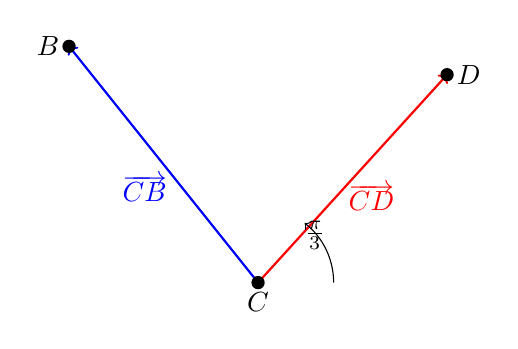
\begin{tikzpicture}[scale=1.2]
    % Define coordinates
    \coordinate (C) at (0,0);
    \coordinate (B) at (-2, 2.5);
    \coordinate (D) at (2, 2.2);
    
    % Draw vectors from C
    \draw[->, blue, thick] (C) -- (B);
    \draw[->, red, thick] (C) -- (D);
    
    % Draw points
    \fill (C) circle (2pt);
    \fill (B) circle (2pt);
    \fill (D) circle (2pt);
    
    % Labels for points
    \node[below] at (C) {$C$};
    \node[left] at (B) {$B$};
    \node[right] at (D) {$D$};
    
    % Draw angle arc
    \draw[->] (0.8,0) arc (0:52:0.8);
    \node at (0.6, 0.5) {$\frac{\pi}{3}$};
    
    % Label vectors
    \node[blue] at (-1.2, 1) {$\overrightarrow{CB}$};
    \node[red] at (1.2, 0.9) {$\overrightarrow{CD}$};
\end{tikzpicture}
\end{center}

(Note: The angle $BCD$ is the angle at vertex $C$ between rays $CB$ and $CD$.)
\end{problem}

\begin{hint}
Find vectors $\overrightarrow{CB}$ and $\overrightarrow{CD}$ emanating from vertex $C$, then use the dot product formula $\cos\theta = \frac{\vec{u} \cdot \vec{v}}{|\vec{u}||\vec{v}|}$ with $\cos(\pi/3) = 1/2$. Be careful to check that your solution gives a positive value for $1-a$.
\end{hint}

\begin{solution}[Sketch]
Step 1: Find vectors from $C$: 
$\overrightarrow{CB} = \mathbf{b} - \mathbf{c} = -\mathbf{i} + \mathbf{k}$ and $\overrightarrow{CD} = \mathbf{d} - \mathbf{c} = (a-2)\mathbf{i} - \mathbf{j} - \mathbf{k}$.

Step 2: Calculate magnitudes: 
$|\overrightarrow{CB}| = \sqrt{2}$ and $|\overrightarrow{CD}| = \sqrt{(a-2)^2 + 2}$.

Step 3: Dot product: 
$\overrightarrow{CB} \cdot \overrightarrow{CD} = -(a-2) + 0 - 1 = 1 - a$.

Step 4: Use formula with $\cos(\pi/3) = 1/2$:
$1 - a = \sqrt{2} \cdot \sqrt{(a-2)^2 + 2} \cdot \frac{1}{2}$

Step 5: Square both sides: 
$4(1-a)^2 = 2[(a-2)^2 + 2]$, which simplifies to $a^2 = 4$, giving $a = \pm 2$.

Step 6: Check constraint: Since the RHS is positive, we need $1-a > 0$, so $a < 1$. Therefore $a = -2$.
\end{solution}

\vspace{1em}

\begin{problem}[Direction Cosines Sum]
Let $\mathbf{r}$ be a non-zero position vector in three-dimensional space with magnitude $r = |\mathbf{r}|$. Suppose $\mathbf{r}$ makes angles $\alpha$, $\beta$, and $\gamma$ with the positive $x$-axis, $y$-axis, and $z$-axis respectively.

The \textbf{direction cosines} of $\mathbf{r}$ are defined as:
$$l = \cos\alpha, \quad m = \cos\beta, \quad n = \cos\gamma$$

Prove that:
$$l^2 + m^2 + n^2 = 1$$

That is, prove that $\cos^2\alpha + \cos^2\beta + \cos^2\gamma = 1$.
\end{problem}

\begin{hint}
Express direction cosines as ratios of components to magnitude.
\end{hint}

\begin{solution}[Sketch]
$\cos\alpha = \frac{a}{|\mathbf{r}|}$, $\cos\beta = \frac{b}{|\mathbf{r}|}$, $\cos\gamma = \frac{c}{|\mathbf{r}|}$. Sum: $\frac{a^2 + b^2 + c^2}{|\mathbf{r}|^2} = \frac{|\mathbf{r}|^2}{|\mathbf{r}|^2} = 1$.
\end{solution}

\vspace{1em}

\begin{problem}[Section Formula Proof]
Prove that if $C$ divides $AB$ in ratio $m:n$, then $\overrightarrow{OC} = \frac{m\mathbf{a} + n\mathbf{b}}{m+n}$ where $\mathbf{a} = \overrightarrow{OA}$, $\mathbf{b} = \overrightarrow{OB}$.
\end{problem}

\begin{hint}
Use $\overrightarrow{AC} = \frac{n}{m+n}\overrightarrow{AB}$ and vector addition.
\end{hint}

\begin{solution}[Sketch]
Since $\frac{CB}{AC} = \frac{m}{n}$, we have $\overrightarrow{AC} = \frac{n}{m+n}(\mathbf{b} - \mathbf{a})$. Then $\overrightarrow{OC} = \mathbf{a} + \overrightarrow{AC} = \mathbf{a} + \frac{n}{m+n}(\mathbf{b} - \mathbf{a}) = \frac{m\mathbf{a} + n\mathbf{b}}{m+n}$.
\end{solution}

\vspace{1em}

\begin{problem}[Skew or Intersecting Lines]
Consider the two lines:
\begin{align*}
L_1: \quad \mathbf{r} &= \begin{pmatrix} 2 \\ -3 \\ 1 \end{pmatrix} + \lambda \begin{pmatrix} 1 \\ 4 \\ 1 \end{pmatrix} \\
L_2: \quad \mathbf{r} &= \begin{pmatrix} -4 \\ 6 \\ -2 \end{pmatrix} + \mu \begin{pmatrix} 4 \\ -11 \\ 3 \end{pmatrix}
\end{align*}

Determine whether lines $L_1$ and $L_2$ are skew or intersecting.
\end{problem}

\begin{hint}
Check if direction vectors are parallel. If not, solve system to see if it's consistent.
\end{hint}

\begin{solution}[Sketch]
Direction vectors not parallel (check ratios). Solve system: from equations 1 and 3, find $\lambda = 6$, $\mu = 3$. Check equation 2: $4(6) + 11(3) = 57 \neq 9$. System inconsistent, so lines are skew.
\end{solution}

\vspace{1em}

\begin{problem}[Line Through Points, Intersection Check]
A line passes through the points $A(1, 3, -2)$ and $B(2, -1, 5)$.

\begin{enumerate}[label=(\roman*)]
    \item Show that the vector equation of the line $AB$ is given by:
    \[
    \mathbf{r} = (\mathbf{i} + 3\mathbf{j} - 2\mathbf{k}) + \lambda_1 (\mathbf{i} - 4\mathbf{j} + 7\mathbf{k}), \quad \lambda_1 \in \mathbb{R}
    \]

    \item Determine if the point $C(3, 4, 9)$ lies on the line.

    \item Consider a second line with parametric equations $x = 1 - \lambda_2$, $y = 2 + 3\lambda_2$, $z = -1 + \lambda_2$.
    
    Assuming this line is neither parallel nor perpendicular to $AB$, determine whether the two lines intersect or are skew.
\end{enumerate}
\end{problem}

\begin{hint}
(i) Find the direction vector $\overrightarrow{AB}$ and use the point $A$ to write the vector equation.
(ii) Substitute the coordinates of $C$ into the line equation and check if a consistent value of $\lambda_1$ exists for all three components.
(iii) Set the two lines equal component-wise, solve for both parameters, then verify if the solution is consistent across all three equations.
\end{hint}

\begin{solution}[Sketch]
(i) Direction vector: $\overrightarrow{AB} = \mathbf{b} - \mathbf{a} = \begin{pmatrix} 2-1 \\ -1-3 \\ 5-(-2) \end{pmatrix} = \begin{pmatrix} 1 \\ -4 \\ 7 \end{pmatrix} = \mathbf{i} - 4\mathbf{j} + 7\mathbf{k}$. 

Using point $A$ as the position vector: $\mathbf{r} = (\mathbf{i} + 3\mathbf{j} - 2\mathbf{k}) + \lambda_1 (\mathbf{i} - 4\mathbf{j} + 7\mathbf{k})$.

(ii) If $C$ lies on the line: $\begin{pmatrix} 3 \\ 4 \\ 9 \end{pmatrix} = \begin{pmatrix} 1 \\ 3 \\ -2 \end{pmatrix} + \lambda_1 \begin{pmatrix} 1 \\ -4 \\ 7 \end{pmatrix}$.

From $x$-component: $3 = 1 + \lambda_1 \Rightarrow \lambda_1 = 2$.

Check $y$-component: $y = 3 - 4(2) = -5 \neq 4$. Since the $y$-coordinate doesn't match, point $C$ does not lie on the line.

(iii) Line 1: $\mathbf{r}_1 = \begin{pmatrix} 1 \\ 3 \\ -2 \end{pmatrix} + \lambda_1 \begin{pmatrix} 1 \\ -4 \\ 7 \end{pmatrix}$. Line 2: $\mathbf{r}_2 = \begin{pmatrix} 1 \\ 2 \\ -1 \end{pmatrix} + \lambda_2 \begin{pmatrix} -1 \\ 3 \\ 1 \end{pmatrix}$.

Equate components: From $x$: $1 + \lambda_1 = 1 - \lambda_2 \Rightarrow \lambda_1 = -\lambda_2$. From $y$: $3 - 4\lambda_1 = 2 + 3\lambda_2$. Substitute $\lambda_1 = -\lambda_2$: $3 + 4\lambda_2 = 2 + 3\lambda_2 \Rightarrow \lambda_2 = -1$, so $\lambda_1 = 1$.

Check $z$-component: LHS: $-2 + 7(1) = 5$. RHS: $-1 + (-1) = -2$. Since $5 \neq -2$, the system is inconsistent. The lines do not intersect and are not parallel, therefore they are skew.
\end{solution}

\vspace{1em}

\begin{problem}[Line-Sphere Intersection Angle]
Let $S$ be the sphere with center at the origin and equation $x^2 + y^2 + z^2 = 10$.

Let $\ell$ be the line with equation:
\[
\begin{bmatrix} x \\ y \\ z \end{bmatrix} = \begin{bmatrix} 1 \\ 2 \\ 1 \end{bmatrix} + \lambda \begin{bmatrix} 0 \\ 1 \\ -1 \end{bmatrix}
\]

\begin{enumerate}[label=(\roman*)]
    \item Find $A$ and $B$, the points of intersection of $S$ and $\ell$.
    \item Find $\angle AOB$ to the nearest degree, where $O$ is the origin.
\end{enumerate}
\end{problem}

\begin{hint}
(i) Write the line in parametric form ($x = 1$, $y = 2 + \lambda$, $z = 1 - \lambda$), substitute into the sphere equation, and solve the resulting quadratic equation for $\lambda$.
(ii) Use the dot product formula $\cos\theta = \frac{\overrightarrow{OA} \cdot \overrightarrow{OB}}{|\overrightarrow{OA}||\overrightarrow{OB}|}$ to find the angle between the two position vectors.
\end{hint}

\begin{solution}[Sketch]
(i) Parametric form: $x = 1$, $y = 2 + \lambda$, $z = 1 - \lambda$. 

Substitute into $x^2 + y^2 + z^2 = 10$:
$1 + (2+\lambda)^2 + (1-\lambda)^2 = 10$
$1 + 4 + 4\lambda + \lambda^2 + 1 - 2\lambda + \lambda^2 = 10$
$2\lambda^2 + 2\lambda + 6 = 10$
$\lambda^2 + \lambda - 2 = 0$
$(\lambda + 2)(\lambda - 1) = 0$

So $\lambda = 1$ or $\lambda = -2$.

When $\lambda = 1$: $A(1, 3, 0)$. When $\lambda = -2$: $B(1, 0, 3)$.

(ii) $\overrightarrow{OA} = \begin{pmatrix} 1 \\ 3 \\ 0 \end{pmatrix}$, $\overrightarrow{OB} = \begin{pmatrix} 1 \\ 0 \\ 3 \end{pmatrix}$.

$\overrightarrow{OA} \cdot \overrightarrow{OB} = (1)(1) + (3)(0) + (0)(3) = 1$.

$|\overrightarrow{OA}| = \sqrt{1^2 + 3^2 + 0^2} = \sqrt{10}$, $|\overrightarrow{OB}| = \sqrt{1^2 + 0^2 + 3^2} = \sqrt{10}$.

$\cos\theta = \frac{1}{\sqrt{10} \cdot \sqrt{10}} = \frac{1}{10} = 0.1$.

Therefore $\theta = \cos^{-1}(0.1) \approx 84.26^\circ \approx 84^\circ$.
\end{solution}

\vspace{1em}


\begin{problem}[Linear Combination of Vectors]
Consider the following four vectors in three-dimensional space:
\begin{align*}
\mathbf{a} &= 2\mathbf{i} + 3\mathbf{j} + \mathbf{k} \\
\mathbf{b} &= \mathbf{i} - \mathbf{j} + 2\mathbf{k} \\
\mathbf{c} &= -\mathbf{i} + 2\mathbf{j} - \mathbf{k} \\
\mathbf{u} &= 5\mathbf{i} + 5\mathbf{j} + 5\mathbf{k}
\end{align*}

Find the values of the scalars $\lambda$, $\mu$, and $\nu$ that satisfy the equation:
\[
\mathbf{u} = \lambda\mathbf{a} + \mu\mathbf{b} + \nu\mathbf{c}
\]

\textit{Note: This means expressing vector $\mathbf{u}$ as a linear combination of vectors $\mathbf{a}$, $\mathbf{b}$, and $\mathbf{c}$. Any vector in 3D space can be written as a combination of three non-coplanar (non-parallel) vectors.}
\end{problem}

\begin{hint}
Substitute the given vectors into the equation $\mathbf{u} = \lambda\mathbf{a} + \mu\mathbf{b} + \nu\mathbf{c}$, then equate the coefficients of $\mathbf{i}$, $\mathbf{j}$, and $\mathbf{k}$ to form a system of three linear equations. Solve the system by elimination.
\end{hint}

\begin{solution}[Sketch]
Substituting: $5\mathbf{i} + 5\mathbf{j} + 5\mathbf{k} = \lambda(2\mathbf{i} + 3\mathbf{j} + \mathbf{k}) + \mu(\mathbf{i} - \mathbf{j} + 2\mathbf{k}) + \nu(-\mathbf{i} + 2\mathbf{j} - \mathbf{k})$.

Equating coefficients gives the system:
\begin{align*}
2\lambda + \mu - \nu &= 5 \quad (1) \\
3\lambda - \mu + 2\nu &= 5 \quad (2) \\
\lambda + 2\mu - \nu &= 5 \quad (3)
\end{align*}

Subtract (1) from (3): $-\lambda + \mu = 0 \Rightarrow \lambda = \mu$.

Substitute $\mu = \lambda$ into (2): $3\lambda - \lambda + 2\nu = 5 \Rightarrow 2\lambda + 2\nu = 5 \Rightarrow \lambda + \nu = \frac{5}{2}$.

Substitute $\mu = \lambda$ into (1): $2\lambda + \lambda - \nu = 5 \Rightarrow 3\lambda - \nu = 5$.

Add these two results: $4\lambda = \frac{5}{2} + 5 = \frac{15}{2} \Rightarrow \lambda = \frac{15}{8}$.

Since $\lambda = \mu$: $\mu = \frac{15}{8}$.

From $3\lambda - \nu = 5$: $\nu = 3 \cdot \frac{15}{8} - 5 = \frac{45}{8} - \frac{40}{8} = \frac{5}{8}$.

Therefore: $\lambda = \frac{15}{8}$, $\mu = \frac{15}{8}$, $\nu = \frac{5}{8}$.
\end{solution}

\begin{takeaways}
\textbf{Key Concepts:}
\begin{itemize}
    \item \textbf{Linear Combination of Vectors:} Any vector can potentially be expressed as a linear combination of other vectors: $\mathbf{v} = \lambda\mathbf{u}_1 + \mu\mathbf{u}_2 + \nu\mathbf{u}_3$. The scalars $\lambda$, $\mu$, $\nu$ are the coefficients.
    
    \item \textbf{Equating Coefficients Method:} When vectors are expressed in component form (using $\mathbf{i}$, $\mathbf{j}$, $\mathbf{k}$), equate the coefficients of each unit vector separately to create a system of linear equations.
    
    \item \textbf{Solving Linear Systems:} The systematic approach involves:
    \begin{enumerate}
        \item Look for relationships by adding/subtracting equations
        \item Find simple relationships (e.g., $\lambda = \mu$) to reduce variables
        \item Substitute to eliminate variables progressively
        \item Solve for remaining variables and back-substitute
    \end{enumerate}
    
    \item \textbf{Verification Strategy:} Always substitute final values back into the original equations to verify correctness. Here: $2(\frac{15}{8}) + \frac{15}{8} - \frac{5}{8} = \frac{30 + 15 - 5}{8} = \frac{40}{8} = 5$ \checkmark
    
    \item \textbf{Linear Independence:} The fact that a unique solution exists ($\lambda = \mu = \frac{15}{8}$, $\nu = \frac{5}{8}$) indicates that the three given vectors are linearly independent and span $\mathbb{R}^3$. Any vector in 3D space can be expressed as a linear combination of these three vectors.
\end{itemize}
\end{takeaways}

\vspace{1em}

\begin{problem}[Parallelogram Fourth Vertex]
Three vertices of a parallelogram are $O(0,0,0)$, $A(2,2,1)$, $B(1,2,2)$. Find all possible positions of the fourth vertex.

\begin{center}
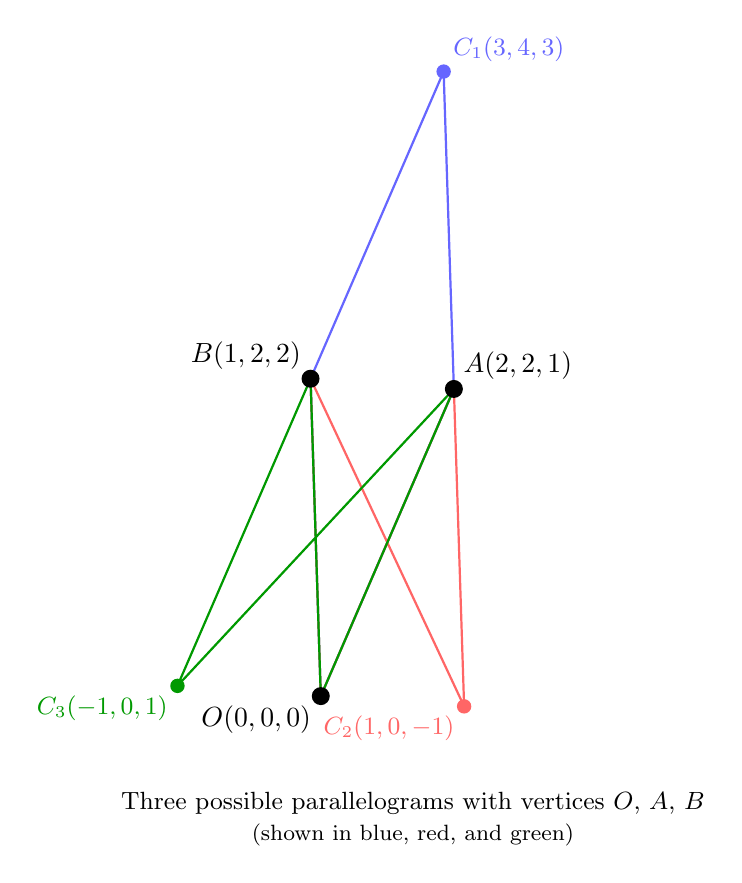
\begin{tikzpicture}[scale=1.3, x={(0.9cm, 0.3cm)}, y={(0cm, 1cm)}, z={(-0.5cm, 0.4cm)}]
    % Define the three given points
    \coordinate (O) at (0, 0, 0);
    \coordinate (A) at (2, 2, 1);
    \coordinate (B) at (1, 2, 2);
    
    % Calculate three possible fourth vertices
    \coordinate (C1) at (3, 4, 3);  % Case 1: C opposite to O
    \coordinate (C2) at (1, 0, -1); % Case 2: C opposite to B
    \coordinate (C3) at (-1, 0, 1); % Case 3: C opposite to A
    
    % Draw Case 1: OABC1 (C1 opposite to O) - blue
    \draw[thick, blue!60] (O) -- (A) -- (C1) -- (B) -- cycle;
    \fill[blue!60] (C1) circle (2pt);
    \node[above right, blue!60, font=\small] at (C1) {$C_1(3,4,3)$};
    
    % Draw Case 2: OACB (C2 opposite to B) - red
    \draw[thick, red!60] (O) -- (A) -- (C2) -- (B) -- cycle;
    \fill[red!60] (C2) circle (2pt);
    \node[below left, red!60, font=\small] at (C2) {$C_2(1,0,-1)$};
    
    % Draw Case 3: OBAC3 (C3 opposite to A) - green
    \draw[thick, green!60!black] (O) -- (B) -- (C3) -- (A) -- cycle;
    \fill[green!60!black] (C3) circle (2pt);
    \node[below left, green!60!black, font=\small] at (C3) {$C_3(-1,0,1)$};
    
    % Draw and label the three given points
    \fill[black] (O) circle (2.5pt);
    \fill[black] (A) circle (2.5pt);
    \fill[black] (B) circle (2.5pt);
    \node[below left, black] at (O) {$O(0,0,0)$};
    \node[above right, black] at (A) {$A(2,2,1)$};
    \node[above left, black] at (B) {$B(1,2,2)$};
    
    % Add annotation
    \node[font=\small, align=center] at (1, -1.5, 0) {
        Three possible parallelograms with vertices $O$, $A$, $B$\\
        {\footnotesize (shown in blue, red, and green)}
    };
\end{tikzpicture}
\end{center}
\end{problem}

\begin{hint}
Consider three cases: which point is opposite to which, giving three parallelograms.
\end{hint}

\begin{solution}[Sketch]
Given three vertices $O(0,0,0)$, $A(2,2,1)$, and $B(1,2,2)$, we need to find all possible fourth vertices $C$ such that $OABC$ forms a parallelogram (in some order).

In a parallelogram, opposite sides are equal and parallel. This gives us three distinct cases depending on which vertex is opposite to which.

\textbf{Case 1: $C_1$ opposite to $O$ (parallelogram $OABC_1$ with $OA \parallel BC_1$ and $OB \parallel AC_1$)}

Using the parallelogram property: $\overrightarrow{OC_1} = \overrightarrow{OA} + \overrightarrow{OB}$.

Calculate:
\begin{align*}
\overrightarrow{OA} &= (2, 2, 1) \\
\overrightarrow{OB} &= (1, 2, 2) \\
\overrightarrow{OC_1} &= (2, 2, 1) + (1, 2, 2) = (3, 4, 3)
\end{align*}

Therefore, $C_1 = (3, 4, 3)$.

\textbf{Verification:} $\overrightarrow{OA} = (2,2,1)$ and $\overrightarrow{BC_1} = (3,4,3) - (1,2,2) = (2,2,1)$ \checkmark

\textbf{Case 2: $C_2$ opposite to $B$ (parallelogram $OAC_2B$ with $OA \parallel C_2B$ and $OC_2 \parallel AB$)}

Using the parallelogram property: $\overrightarrow{OC_2} = \overrightarrow{OA} - \overrightarrow{OB}$.

Calculate:
\begin{align*}
\overrightarrow{OC_2} &= (2, 2, 1) - (1, 2, 2) = (1, 0, -1)
\end{align*}

Therefore, $C_2 = (1, 0, -1)$.

\textbf{Verification:} $\overrightarrow{OA} = (2,2,1)$ and $\overrightarrow{C_2B} = (1,2,2) - (1,0,-1) = (0,2,3)$... Actually, $\overrightarrow{AC_2} = (1,0,-1) - (2,2,1) = (-1,-2,-2)$ and $\overrightarrow{OB} = (1,2,2)$. Let me verify: $\overrightarrow{OC_2} + \overrightarrow{OB} = (1,0,-1) + (1,2,2) = (2,2,1) = \overrightarrow{OA}$ \checkmark

\textbf{Case 3: $C_3$ opposite to $A$ (parallelogram $OBC_3A$ with $OB \parallel C_3A$ and $OC_3 \parallel BA$)}

Using the parallelogram property: $\overrightarrow{OC_3} = \overrightarrow{OB} - \overrightarrow{OA}$.

Calculate:
\begin{align*}
\overrightarrow{OC_3} &= (1, 2, 2) - (2, 2, 1) = (-1, 0, 1)
\end{align*}

Therefore, $C_3 = (-1, 0, 1)$.

\textbf{Verification:} $\overrightarrow{OB} = (1,2,2)$ and $\overrightarrow{C_3A} = (2,2,1) - (-1,0,1) = (3,2,0)$... Let me verify: $\overrightarrow{OC_3} + \overrightarrow{OA} = (-1,0,1) + (2,2,1) = (1,2,2) = \overrightarrow{OB}$ \checkmark

\textbf{Final Answer:} The three possible positions for the fourth vertex are:
$$C_1 = (3, 4, 3), \quad C_2 = (1, 0, -1), \quad C_3 = (-1, 0, 1)$$
\end{solution}

\vspace{1em}
